%%%%%%%% ICML 2026 实验报告 — 国标麻将 AI %%%%%%%%%%%%%%%%%

\documentclass{article}

% ICML 2026 模板
\usepackage[accepted]{icml2026}

% 中文支持 (XeLaTeX)
\usepackage{fontspec}
\usepackage{xeCJK}
\setCJKmainfont{Songti SC}
\setCJKsansfont{PingFang SC}
\setCJKmonofont{PingFang SC}

% 数学与排版
\usepackage{microtype}
\usepackage{graphicx}
\usepackage{booktabs}
\usepackage{amsmath}
\usepackage{amssymb}
\usepackage{mathtools}
\usepackage{hyperref}
\usepackage{tikz}
\usepackage{xcolor}
\usepackage{float}
\usepackage{setspace}
\setstretch{1.08}
\AtBeginDocument{\small}
\usetikzlibrary{arrows.meta, positioning, shapes, calc, fit, backgrounds}

% 引用
\usepackage[capitalize,noabbrev]{cleveref}

% 自定义颜色
\definecolor{cnnblue}{HTML}{4472C4}
\definecolor{segreen}{HTML}{70AD47}
\definecolor{lstmred}{HTML}{E74C3C}
\definecolor{fusionpurple}{HTML}{9B59B6}
\definecolor{ttagold}{HTML}{F39C12}
\definecolor{lightgray}{HTML}{F2F2F2}

% 运行标题
\icmltitlerunning{ZZMahjongBot}

\begin{document}

\twocolumn[
  \icmltitle{ZZMahjongBot}

  \begin{icmlauthorlist}
    \icmlauthor{陈治中 2500012905}{pku}
  \end{icmlauthorlist}

  \icmlaffiliation{pku}{北京大学, 北京, 中国}

  \vskip 0.15in
  \begin{center}
  \small
  Botzone 最终积分赛 bot 版本排名 17，分数 1289\\
  Botzone 最后一次模拟赛 bot 版本排名 11，分数 1410\\
  2026.6.28\\
  \url{https://github.com/flowwalker/ZZmahjongBot}
  \end{center}

  \icmlkeywords{Mahjong, Data Augmentation, Test-Time Augmentation, CNN, Group Theory, SE-Net}

  \vskip 0.3in
]

\printAffiliationsAndNotice{}

\begin{abstract}
国标麻将是具有$10^{48}$状态空间、235维离散动作空间的不完全信息四人博弈。

笔者将通过自己对架构、特征工程、数据增强、以及数据增强后因效率低下而进行的预处理优化的探索实验和分析，来展示自己的思考和创新性，和自己的想法对于麻将bot设计的意义。受限于期末周时间紧迫和资金算力不足，笔者探索的大多架构大多是实验性的（而非疯狂调参竞赛性的），重点训了个别时间预算合适的架构，然而不少因为超参调节缺乏时间原因而失败。经历长时间探索，最终得出几个较有前景的架构思想，以及几个能够botzone实战不错的完整bot，详见下解。
\end{abstract}

%===========================================================================
\section{引言}
%===========================================================================

国标麻将是国家体育总局1998年颁布的竞技麻将规则，包含81种番型，和牌门槛8番起和。作为四人不完全信息博弈，Bot系统面临三个核心挑战：
(1) 采取怎样的架构和使用如何的特征最有利于bot学到胡牌的价值和技巧而非随机的噪音；
(2) (2) 如何在有限训练数据下实现充分利用与避免过拟合；
(3) (3) 如何在Botzone 6秒、单核CPU时限内做出最优决策。

不同于大型比赛中动不动就是几十天的训练只为最终结果，我的本次探索力求

(1) 在极有限算力下进行我认为能系统的探索——覆盖特征、模型、数据、训练、部署五个维度的提升措施和思想；

(2) 探寻对于提升Bot真正有帮助的关键创新点

(3) 给出实验中遇到的``理想美好，实际骨感''的现象记录与分析

(4) 简明介绍自己花最多时间的的feature和model架构的探索历程

为了创新性展示和完整性展示充分兼顾，本文前段先重点介绍自己对于麻将bot的创新理论点，然后详细介绍自己对feature和model维度的完整探索历程，其余可详见code文件包或者我的GitHub仓库。

注：由于第一次在华为云平台训练模型没有经验，很多acc和loss日志丢失且未记录，具体数据以下大多为个人实验后印象。

%===========================================================================
\section{关键创新点}
%===========================================================================

%---------------------------------------------------------------------------
\subsection{创新一：SE通道注意力机制}
%---------------------------------------------------------------------------

Squeeze-and-Excitation (SE) 通道注意力是我从纯CNN走向``打牌有点感觉''的\textbf{第一个转折点}。

感觉上，在最初的3层纯CNN上，模型对所有输入通道一视同仁——手牌的4个通道与门风的1个通道在卷积核眼中没有区别。SE模块对每个通道做全局平均池化(GAP)，经两层全连接网络学习通道间依赖关系，输出0--1权重向量，逐通道缩放原始特征图：

\begin{equation}
\text{SE}(\mathbf{X}) = \mathbf{X} \odot \sigma\big(\mathbf{W}_2 \cdot \text{Mish}(\mathbf{W}_1 \cdot \text{GAP}(\mathbf{X}))\big)
\end{equation}

\begin{figure}[ht]
\begin{center}
\resizebox{0.42\columnwidth}{!}{%
\begin{tikzpicture}[node distance=0.35cm, auto,
  block/.style={rectangle, draw, rounded corners, minimum width=1.8cm, minimum height=0.5cm, font=\footnotesize, align=center},
  arrow/.style={-{Stealth}, thick}]

\node[block, fill=cnnblue!15] (input) {$\mathbf{X}$: $C\!\times\!H\!\times\!W$};
\node[block, fill=lightgray, below=0.3cm of input] (gap) {GAP: $C\!\times\!1\!\times\!1$};
\node[block, fill=segreen!15, below=0.3cm of gap] (fc1) {FC+Mish: $C/16$};
\node[block, fill=segreen!15, below=0.3cm of fc1] (fc2) {FC+Sigmoid: $C$};
\node[block, fill=cnnblue!15, below=0.3cm of fc2] (scale) {$\mathbf{X}\!\odot\!\text{weight}$};
\node[block, fill=cnnblue!15, below=0.3cm of scale] (output) {输出: $C\!\times\!H\!\times\!W$};

\draw[arrow] (input) -- (gap);
\draw[arrow] (gap) -- (fc1);
\draw[arrow] (fc1) -- (fc2);
\draw[arrow] (fc2) -- (scale);
\draw[arrow] (input.east) -- ++(0.3,0) |- (scale.east);
\draw[arrow] (scale) -- (output);
\end{tikzpicture}%
}
\caption{SE模块。右路跳跃连接表示残差：原始特征与通道权重逐元素相乘。}
\label{fig:se}
\end{center}
\end{figure}

以我最终设计的160个通道为例，手牌(4ch)、弃牌历史(112ch)、对手鸣牌(21ch)在不同决策场景下重要性迥异。SE让模型\emph{自行学习}注意力分布。引入SE使得胡牌水平有明显的提高，而计算开销仅$O(C^2/r)$，可谓十分划算。

%---------------------------------------------------------------------------
\subsection{创新二：特征工程的极致压榨}
%---------------------------------------------------------------------------

特征空间经历了\textbf{6ch $\rightarrow$ 16ch $\rightarrow$ 148ch $\rightarrow$ 224ch(放弃) $\rightarrow$ 155ch $\rightarrow$ 160ch}周期。

\textbf{飞跃点在148ch}。核心变化是弃牌序列从4ch快照扩展为\textbf{4家$\times$28步完整弃牌历史}（112ch），从后来的对局感觉上，放炮的概率显著降低，推测原因是\textbf{有了更多的序列记忆当然更容易避免对方的心思}。（当然也增加了很多精细化的特征，详见下表。）

同时手牌改为1--4张分层编码，鸣牌细化为16ch。

\textbf{最终的平衡是160ch}。经历224ch膨胀失败（预计算时间爆炸）后，最终收敛到160ch：

\begin{table}[ht]
\caption{160ch最终特征通道组成}
\label{tab:channels}
\begin{center}
\footnotesize
\begin{tabular}{lp{0.7cm}p{3.6cm}}
\toprule
通道 & ch & 内容 \\
\midrule
0--3   & 4   & 手牌：1--4张分层编码 \\
4--7   & 4   & \textbf{明牌：手牌+场上可见（小巧思，揣摩对方心思——增强防御性）} \\
8--28  & 21  & 鸣牌：4家$\times$5(吃向/碰/明杠)+暗杠 \\
29--32 & 4   & 圈风 one-hot \\
33--36 & 4   & 门风 one-hot \\
37--40 & 4   & 牌墙剩余归一化 \\
41--152 & \textbf{112} & \textbf{弃牌历史：4家$\times$28步打点} \\
153    & 1   & \textbf{当前待决策牌（小巧思，不增加计算基础上加快学习，下同）} \\
154    & 1   & 牌来源方 \\
155    & 1   & 牌墙最后一张标志 \\
156    & 1   & 刚杠标志 \\
157--159 & 3 & 对手手牌数 \\
\bottomrule
\end{tabular}
\end{center}
\end{table}

这里的160ch只包含\emph{直接可观测}的游戏状态——不做任何语义预处理。将``理解''任务完全交给神经网络。

我最最最核心的想法是，由于时间原因，增加到224ch计算带来时间开销十分不划算，\textbf{因此秉承``特征为所见''的思想}不断扩增到160ch，且均确保为无需大处理的特征。

%---------------------------------------------------------------------------
\subsection{创新三$\boldsymbol{\&}$四：TTA + 三模型全局软平均投票}
%---------------------------------------------------------------------------

这里有一个风险是需要修改main函数，因此中间折腾了一段时间，但从结果看还是有一定效果的。

\textbf{而我也认为这是我最有创新的点子！}

TTA（测试时增强）和多模型投票在部署中\textbf{协同工作}。TTA对同一局面随机采样$N_{\text{TTA}}$个对称变换分别推理后取平均；多模型投票利用3个独立训练模型（同架构、不同随机种子）的多样性。最终方案为\textbf{全局软平均}——将所有模型$\times$所有变换的logits直接取平均后argmax：

\begin{equation}
\text{action} = \arg\max \frac{1}{|\mathcal{M}| \times N_{\text{TTA}}} \sum_{m \in \mathcal{M}} \sum_{t=1}^{N_{\text{TTA}}} f_m\big(T_t(x)\big)
\end{equation}

软平均保留logit分布的完整信息，对模型间置信度差异更鲁棒——一个过于自信的错误模型在硬投票中与正确模型同等权重，在软平均中会被部分稀释。

这里当然也要考虑过其他的例如rms和vote走法，可见后文提及放弃原因。

\begin{figure}[ht]
\begin{center}
\resizebox{0.96\columnwidth}{!}{%
\begin{tikzpicture}[node distance=0.6cm, auto,
  block/.style={rectangle, draw, rounded corners, minimum width=3cm, minimum height=0.6cm, font=\footnotesize, align=center},
  smallblock/.style={rectangle, draw, rounded corners, minimum width=2.2cm, minimum height=0.55cm, font=\footnotesize, align=center},
  arrow/.style={-{Stealth}, thick}]

\node[block, fill=lightgray] (obs) {观测 $x$ (160ch $\times$ 4 $\times$ 9)};
\node[block, fill=ttagold!15, below=0.6cm of obs] (tta) {TTA: 随机采样50个变换};
\node[block, fill=cnnblue!15, below left=0.7cm and 1.4cm of tta] (m1) {模型1};
\node[block, fill=segreen!15, below=0.7cm of tta] (m2) {模型2};
\node[block, fill=lstmred!15, below right=0.7cm and 1.4cm of tta] (m3) {模型3};
\draw[arrow] (obs) -- (tta);
\draw[arrow] (tta.south) -- ++(0,-0.1) -| (m1);
\draw[arrow] (tta.south) -- ++(0,-0.1) -| (m2);
\draw[arrow] (tta.south) -- ++(0,-0.1) -| (m3);

\node[smallblock, fill=lightgray, below=0.6cm of m1] (l1) {logits$_1^{1..50}$};
\node[smallblock, fill=lightgray, below=0.6cm of m2] (l2) {logits$_2^{1..50}$};
\node[smallblock, fill=lightgray, below=0.6cm of m3] (l3) {logits$_3^{1..50}$};
\draw[arrow] (m1) -- (l1);
\draw[arrow] (m2) -- (l2);
\draw[arrow] (m3) -- (l3);

\node[block, fill=fusionpurple!15, below=1.5cm of m2] (avg) {全局软平均: $\frac{1}{150}\sum$logits};
\draw[arrow] (l1.south) |- (avg);
\draw[arrow] (l2.south) -- (avg);
\draw[arrow] (l3.south) |- (avg);

\node[block, fill=cnnblue!15, below=0.6cm of avg] (out) {argmax $\rightarrow$ 动作};
\draw[arrow] (avg) -- (out);
\end{tikzpicture}%
}
\caption{TTA + 多模型投票推理管线。$3\times50=150$次前向($\sim$2.25s)，logits全局平均后argmax。}
\label{fig:tta_vote}
\end{center}
\end{figure}

\textbf{这里的动机是：因为不能确保每一个模型在任何情况下都确保正确，且``训练时模型并未见过足够多的市面''，这样就需要临时增强取平均来减少一下方差，使得模型更加稳健}

实测出来的效果是，对于复试对局：连赢四盘的概率增加（稳健），但也开始在某些情况出现了过于保守的打牌方式。

%---------------------------------------------------------------------------
\subsection{创新五：模型架构的系统探索}
%---------------------------------------------------------------------------

共探索3款，11个架构。本节聚焦两个最重要的创新；完整演进见第\ref{sec:evolution}节。

\subsubsection*{金字塔CNN-SE (v8)：最终部署模型}

\begin{figure}[ht]
\begin{center}
\resizebox{0.96\columnwidth}{!}{%
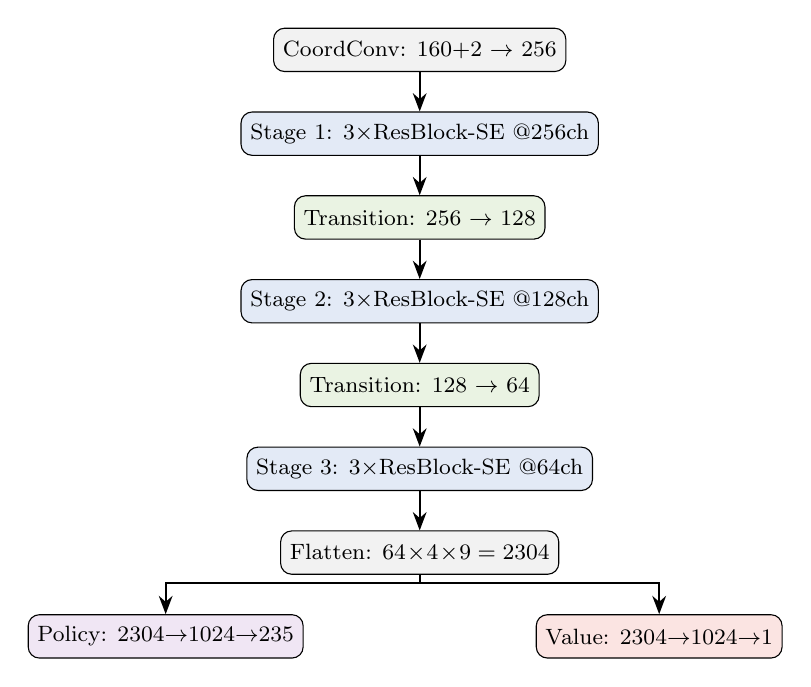
\begin{tikzpicture}[node distance=0.6cm, auto,
  block/.style={rectangle, draw, rounded corners, minimum width=2.8cm, minimum height=0.55cm, font=\footnotesize, align=center},
  arrow/.style={-{Stealth}, thick}]

\node[block, fill=lightgray] (coord) {CoordConv: 160+2 $\rightarrow$ 256};
\node[block, fill=cnnblue!15, below=0.5cm of coord] (s1) {Stage 1: 3$\times$ResBlock-SE @256ch};
\node[block, fill=segreen!15, below=0.5cm of s1] (t1) {Transition: 256 $\rightarrow$ 128};
\node[block, fill=cnnblue!15, below=0.5cm of t1] (s2) {Stage 2: 3$\times$ResBlock-SE @128ch};
\node[block, fill=segreen!15, below=0.5cm of s2] (t2) {Transition: 128 $\rightarrow$ 64};
\node[block, fill=cnnblue!15, below=0.5cm of t2] (s3) {Stage 3: 3$\times$ResBlock-SE @64ch};
\node[block, fill=lightgray, below=0.5cm of s3] (flat) {Flatten: $64\!\times\!4\!\times\!9 = 2304$};
\node[block, fill=fusionpurple!15, below left=0.5cm and -0.3cm of flat] (phead) {Policy: 2304$\rightarrow$1024$\rightarrow$235};
\node[block, fill=lstmred!15, below right=0.5cm and -0.3cm of flat] (vhead) {Value: 2304$\rightarrow$1024$\rightarrow$1};

\draw[arrow] (coord) -- (s1);
\draw[arrow] (s1) -- (t1);
\draw[arrow] (t1) -- (s2);
\draw[arrow] (s2) -- (t2);
\draw[arrow] (t2) -- (s3);
\draw[arrow] (s3) -- (flat);
\draw[arrow] (flat.south) -- ++(0,-0.1) -| (phead);
\draw[arrow] (flat.south) -- ++(0,-0.1) -| (vhead);
\end{tikzpicture}%
}
\caption{CNN-SE金字塔(v8)。三级256$\rightarrow$128$\rightarrow$64，10.4M参数，flat\_dim仅2304。}
\label{fig:pyramid}
\end{center}
\end{figure}

金字塔的优势：

(1) 多尺度特征——深层捕捉细粒度局部模式，浅层保留粗粒度全局结构；

(2) \textbf{参数效率——flat\_dim从9216降至2304，训练速度大幅加快（这是我最主要的目的）}

注：这里的v头实际无用，因为不进行RL训练，但作为接口保留。

\subsubsection*{Dual Path双路并行}

将时序建模(BiLSTM)和空间建模(CNN)并行化——共享CNN提取底层特征后，分叉为两路独立处理，再通过Transformer融合：

\begin{figure}[ht]
\begin{center}
\resizebox{0.96\columnwidth}{!}{%
\begin{tikzpicture}[node distance=0.7cm, auto,
  block/.style={rectangle, draw, rounded corners, minimum width=2.8cm, minimum height=0.6cm, font=\footnotesize, align=center},
  arrow/.style={-{Stealth}, thick}]

\node[block, fill=cnnblue!15] (shared) {共享CNN: 9$\times$ResBlock-SE @64ch};

\node[block, fill=lstmred!15, below left=0.55cm and -0.6cm of shared] (lstm) {上路: BiLSTM(128,bidir)$\rightarrow$64ch};
\node[block, fill=segreen!15, below right=0.55cm and -0.6cm of shared] (cnn) {下路: CNN Branch @32ch (zero-init)};

\draw[arrow] (shared.south) -- ++(0,-0.15) -| (lstm.north);
\draw[arrow] (shared.south) -- ++(0,-0.15) -| (cnn.north);

\node[block, fill=fusionpurple!15, below=1.2cm of shared] (fusion) {Concat[64+32] + PosEmbed\\4$\times$TransformerBlock(96,4头)};
\draw[arrow] (lstm.south) |- (fusion.west);
\draw[arrow] (cnn.south) |- (fusion.east);

\node[block, fill=lightgray, below=0.55cm of fusion] (head) {Flatten $\rightarrow$ Policy: 3456$\rightarrow$512$\rightarrow$235};
\draw[arrow] (fusion) -- (head);
\end{tikzpicture}%
}
\caption{Dual Path (v9 Dual Light, 3.56M)。上路BiLSTM时序，下路CNN空间，Transformer融合。}
\label{fig:dual}
\end{center}
\end{figure}

下路融合cnn，最主要的目的是并行，避免lstm浪费时间；当然，这也顺便可以视为纯cnn外接lstm时序建模的扩展。

理论上的直觉是：

\begin{itemize}
  \item 空间感觉用时序建模
  \item 空间感觉和时间感觉并行
  \item 注意力自己注意此刻选择何种感觉最为可靠
\end{itemize}

如果不考虑时间，这个架构似乎是最为有效的，与其打牌深感其兵法精妙，奈何lstm在2x数据的训练和lr调节就十分费力。

\textbf{最终选CNN-SE而非Dual Path}我认为是一种务实的权衡：

(1) Dual Path训练耗时是CNN-SE的2--4倍（BiLSTM无法充分利用NPU并行性）；

(2) 同等时间下CNN-SE可跑更多epoch；

(3) 由于更有时间调参以及lr适合，CNN-SE训练稳定性更好。

\textbf{但我仍认为Dual Path在算力充足时是更有潜力的方向（见第\ref{sec:ideal}节）。}

%---------------------------------------------------------------------------
\subsection{创新六：内存预加载}
%---------------------------------------------------------------------------

数据供给速度决定能否达到精度上限。为了节省算力带来的金钱花费，我经历了六代演进：

\begin{center}
\footnotesize
\begin{tabular}{cp{2.8cm}p{3.2cm}}
\toprule
代 & 方案 & NPU利用率 \\
\midrule
v0 & 逐文件np.load，磁盘争抢严重 & 锯齿状，常为0等待 \\
v1 & np.concatenate扁平化 & （没增强）时间略快 \\
v2 & 预处理增强(失败)，磁盘50GB & 一个晚上都加载不完 \\
v3 & LazyAug延迟增强，缓存优化 & 可以加载了，但太慢了 \\
\textbf{v4} & \textbf{MemPreload内存预加载} & \textbf{连续20--40\%} \\
v5 & 分层随机增强（后来无用） & 连续20--40\% \\
\bottomrule
\end{tabular}
\end{center}

\textbf{MemPreloadDataset的核心设计}：

\begin{enumerate}
  \item \textbf{全量内存预分配}：\texttt{np.empty}一次性分配三个连续大数组（int8压缩vs float32爆炸），避免\texttt{np.concatenate}的内存碎片。
  \item \textbf{纯内存索引}：\texttt{\_\_getitem\_\_}退化为int8解码+即时增强变换，训练全程零磁盘I/O。这个是非常之重要的！
  \item LazyAugSampler：按变换分组shuffle。
\end{enumerate}

%===========================================================================
\section{``美好理想$\rightarrow$现实骨感''的崩溃经验}
%===========================================================================

%---------------------------------------------------------------------------
\subsection{``不做选择''全架构拼接野心的悲哀}
\label{sec:fail_fullarch}
%---------------------------------------------------------------------------

\textbf{理想是}：既然BiLSTM擅长时序、Self-Attention擅长全局关联、CNN擅长空间、SE擅长通道——全部拼接在一起！v6 (Gated Fusion,) 和 v7 (Cross-Attention) 通过可学习门控或交叉注意力融合多个分支。

\textbf{但现实}：完全不可训练。无论怎么调学习率、加warmup、降batch size、加Gradient Clipping——loss剧烈振荡，val\_acc始终$\sim$30\%+

推测原因是：

(1) 多分支梯度方向和量级可能造成错配以及巨大的不稳定

(2) 或许交叉注意力训练初期退化为噪声，反向传播污染主干网络；

\textbf{架构复杂度需要与数据和算力匹配}。所以只能说优雅可并行、专注的设计远比复杂、全面的设计有优势。

%---------------------------------------------------------------------------
\subsection{v头的麻烦}
\label{sec:fail_rl}
%---------------------------------------------------------------------------

\textbf{正常的理想}：我的想法，或者说正常人都会想，SL预训练后，PPO自我对弈微调——模型在与自己博弈中超越人类数据。

现实是v头太难搞了。

三个失败的尝试：

\textbf{(1) Value Head干扰Policy}：SL只优化Policy Head，Value Head随机初始化。首次RL更新value\_loss$\approx$12,000——崩。

\textbf{(2) 算力时间不足}：从头训根本是天方夜谈，更何况是时间紧迫的期末周。

\textbf{(3) SL阶段v头不可训}：纵使是sl阶段利用稀疏的结果score进行奖励，也完全没法让bot懂得什么好什么坏，只知道什么结束了，v头照样爆。

rl放弃。

%---------------------------------------------------------------------------
\subsection{12$\times$增强的过拟合}
%---------------------------------------------------------------------------

实验12x数据增强的时候遇到了如下几个问题：（首先核心是时间翻了12倍）

\begin{itemize}
  \item 学习率未改变直接改成12x，发现第二个epoch就过拟合了
  \item 调小lr重训发现acc涨得太慢了，根本没时间收敛
  \item 又稍微调高lr，结果又过拟合了。
  \item 尝试在第一个epoch后调小lr微调，也过拟合。
\end{itemize}

推测原因是，全排列6x似乎有点让模型矫枉过正，提供过多重复样本而容易导致过拟合。但后来没有时间没有进一步实验了。比赛直接采用2x。

%---------------------------------------------------------------------------
\subsection{准确率的抛物线怪象}
%---------------------------------------------------------------------------

直觉上理论上应该是过拟合后acc微微下降，但麻将训练是过拟合后立刻暴跌，很反直觉。

猜测是面对``无能局面''（无论选什么动作都输）时，人类动作本质随机。模型过拟合时开始``记忆''这些随机标签。

%---------------------------------------------------------------------------
\subsection{288$\times$随机增强是个``灾难''}
\label{sec:fail_288}
%---------------------------------------------------------------------------

激动的尝试288x，因为\textbf{288x包含着我对箭牌和风牌数据增强的良苦创新，课件只提供了12x增强的想法}

结果一天的金钱和时间离我而去。后来立刻意识到应该先做2x估算288x时间，一算发现1epoch都要上几十天。

于是进行了\textbf{三种尝试}想充分利用288x：怀着认为利用随机性让他充分见到各种增强的局面。

(1) 跨batch随机4$\times$——几乎零提升；

(2) batch内逐个随机变换——略有下降；

(3) batch内逐个随机5$\times$——val\_acc暴跌至$\sim$30\%。灾难！

推测的\textbf{原因}：增强的核心价值是让模型看到\emph{同一局面的不同对称版本}。batch内每个样本使用不同随机变换时，模型看到的是混乱信号——不同变换对同一局面产生矛盾梯度更新。

因此，最终认为增强的``多样性''需要与``一致性''平衡。我采取方案先（固定2$\times$ + 同batch同变换 + GroupNorm）再尝试12x等等（如果有时间的话，而事实上无）

%---------------------------------------------------------------------------
\subsection{十分之困惑：Botzone超时与不超时}
\label{sec:fail_timeout}
%---------------------------------------------------------------------------

使用$N_{\text{TTA}}\!=\!50$，自行测试两天\textbf{零超时}（有对局记录为证，不可深究-serious-版本14），但正式计分赛时有超时崩溃扣分，非常让人困惑。

我的推测：计分赛平台同时运行大量对局，CPU资源被争抢，单核性能下降——
\textbf{所以感觉是Botzone缺乏资源隔离机制问题，若不然我的成绩必然能达到一个更高的水平。}

%---------------------------------------------------------------------------
\subsection{224ch专家特征的Python瓶颈}
\label{sec:fail_224ch}
%---------------------------------------------------------------------------

\textbf{理想情况是}：将牌效分析、安全度、听牌判断等专家知识编码为额外76ch特征(224ch)，让模型不需要学习已知规律。

\textbf{但现实}：通过Python版MahjongFanCalculator实时计算番型，单次\texttt{\_update\_obs()}耗时约数百毫秒。一局100--200次决策需数十秒预处理。490万样本的预处理时间远超NPU训练时间。（当然也可能是因为这部分处理算法后来就没有深入研究）

只能说有点讽刺：添加专家特征是为了``省训练时间''，但Python预处理耗时远超模型学习这些规律所需的时间。

%---------------------------------------------------------------------------
\subsection{关于数据增强时均值的选择——主要是rms的失败}
%---------------------------------------------------------------------------

当时考虑过如下几个方案：

\begin{itemize}
  \item 采用vote走法，选投票最多的走法——但考虑到很大可能每个增强情况想法不同，且动作空间不小，可能都差不多导致失效，但未来可能可以尝试
  \item rms，即采用平方平均值来替代vote软平均，动机是：平方可以增大正确的量级、缩小不合适的走法量级，但是实际效果暴跌——推测是
  \begin{itemize}
    \item 平方可以增大正确量级也会\textbf{放大盲目自信的量级}因此造成不稳定
    \item 平方后概率不归一化，可能造成奇怪现象
  \end{itemize}
\end{itemize}

%===========================================================================
\section{最终方案与理想方案}
%===========================================================================

%---------------------------------------------------------------------------
\subsection{最终提交的Botzone版本}
%---------------------------------------------------------------------------

综合所有约束和实验结果：

\begin{center}
\footnotesize
\begin{tabular}{lp{5.5cm}}
\toprule
组件 & 选择 \\
\midrule
特征 & 160ch，仅直接可观测信息 \\
模型 & CNN-SE Pyramid (v8) \\
增强 & 2$\times$分层增强（数字对称$\mathbb{Z}_2$） \\
数据 & int8压缩，33GB内存预加载 \\
训练 & Adam+CosineAnnealing+LabelSmooth \\
部署 & 3模型$\times$50 TTA软平均投票（测试赛不加更佳） \\
\bottomrule
\end{tabular}
\end{center}

%---------------------------------------------------------------------------
\subsection{理想中的无限资源训练流程}
\label{sec:ideal}
%---------------------------------------------------------------------------

如果时间、金钱、算力均无约束，

\begin{center}
\footnotesize
\begin{tabular}{lp{5.2cm}}
\toprule
组件 & 选择 \\
\midrule
特征 & 160ch，仅直接可观测信息（甚至224ch预处理，关键在时间） \\
模型 & \textbf{CNN-SE Pyramid-双路(Bilstm/零权重cnn)-transformer} \\
增强 & \textbf{288$\times$全分层增强+精细的lr调节匹配} \\
数据 & int8压缩，内存预加载 \\
训练 & Adam+CosineAnnealing \\
部署 & \textbf{k模型$\times$n TTA软平均投票}（多轮测试选最佳方案） \\
\bottomrule
\end{tabular}
\end{center}

小可能：利用sl好的此模型当老师，用于快速提升rl模型，随后让rl进行自对弈。

%===========================================================================
\section{探索历程：Feature与Model的演进}
\label{sec:evolution}
%===========================================================================

%---------------------------------------------------------------------------
\subsection{特征工程演进 (features/)}
%---------------------------------------------------------------------------

\textbf{v1\_6ch\_minimal.py} — 起点：门风+圈风+手牌(4ch堆叠)，无弃牌/鸣牌/牌墙。（提供的sample）

\textbf{v2\_16ch\_visible.py} — 睁开双眼：+弃牌标记(4ch)+鸣牌(4ch)+明牌(1ch)+牌墙(1ch)。首个``可用''版本。

\textbf{v3\_148ch\_discard\_history.py} — \textbf{质的飞跃}：弃牌序列4ch$\rightarrow$112ch（4家$\times$28步完整历史），手牌分层编码，鸣牌16ch。设计洞察：弃牌顺序和节奏蕴含对手手牌倾向。

\textbf{v4\_224ch\_semantic.py} — 膨胀顶点：+76ch语义+专家特征。因Python预处理瓶颈被放弃（见第\ref{sec:fail_224ch}节）。

\textbf{v5\_155ch\_aux\_state.py} — 返璞归真：+7ch辅助状态（待决策牌、牌来源、手牌数等）。降低模型推断负担。

\textbf{v6\_160ch\_meld21.py} — \textbf{最终收敛}：+5ch MELD精细化（吃牌左/中/右方向编码，暗杠独立）。``直接可观测信息''路线的终稿。

\begin{table}[ht]
\caption{特征工程演进}
\label{tab:feature_evo}
\begin{center}
\footnotesize
\begin{tabular}{lcl}
\toprule
版本 & ch & 核心变化 \\
\midrule
v1 & 6   & 手牌+风位，sample基本可用 \\
v2 & 16  & +弃牌/鸣牌/牌墙，首个可用 \\
v3 & 148 & \textbf{112ch弃牌历史和更多精细特征，飞跃} \\
v4 & 224 & +76ch非常耗时间的专家语义，被放弃 \\
v5 & 155 & +7ch辅助状态 \\
\textbf{v6} & \textbf{160} & \textbf{+5ch更精细，最终方案} \\
\bottomrule
\end{tabular}
\end{center}
\end{table}

%---------------------------------------------------------------------------
\subsection{模型架构演进 (models/)}
%---------------------------------------------------------------------------

\subsubsection*{第一阶段：纯CNN探索 (v1--v3)}

\textbf{v1}：3层Conv2d，sample。\textbf{v2}：\textbf{首次引入SE+CoordConv+Mish+GroupNorm}，效果显著提升，SE自注意力非常有帮助。\textbf{v3}：v2的16块ResBlock放大版，验证了``更大不等于更好''，所以后期不再一味尝试堆大模型。

\subsubsection*{第二阶段：序列建模与膨胀 (v4--v7)}

\textbf{v4\_bilstm\_sa\_148ch.py}：CNN+SE串接BiLSTM(128,bidir)+SelfAttention(256,8头)。\textbf{效果最优}——实战和牌和出牌技巧优于同期CNN-SE。但训练耗时是CNN-SE的3--4倍，在数据增强时不够时间调参和训好。

\textbf{v5\_dual\_tower\_224ch.py}：策略/价值双塔独立。稍微尝试训练发散失败。\textbf{v6\_gated\_fusion\_224ch.py}：门控融合，未实验。\textbf{v7\_multibranch\_cross\_attn\_224ch.py}：Cross-Attention融合(158M)，完全不收敛（见第\ref{sec:fail_fullarch}节）。

\subsubsection*{第三阶段：回归与收敛 (v8)}

\textbf{v8\_cnn\_se\_pyramid\_160ch.py：最终部署模型}。16块平坦256ch$\rightarrow$9块金字塔(256$\rightarrow$128$\rightarrow$64)（前面提到过的省参数，加训练速度）

\subsubsection*{第四阶段：新型架构探索 (v9--v11)}

\textbf{v9\_dual\_light\_160ch.py}：Dual Path轻量版。水平与CNN-SE相当但不够稳定。但因为是light可以理解

\textbf{v10\_dual\_zerocnn\_160ch.py}：消融版，未实验。\textbf{v11\_cnn\_transformer\_160ch.py}：CNN金字塔+Transformer，未实验。

\begin{table}[ht]
\caption{模型架构演进全景}
\label{tab:model_evo}
\begin{center}
\footnotesize
\begin{tabular}{llcl}
\toprule
版本 & 架构 & 参数 & 状态 \\
\midrule
v1  & 3层CNN, 6ch & 0.7M & 起点 \\
v2  & CNN-SE 4Block & $\sim$3M & 引入SE \\
v3  & CNN-SE Large & $\sim$29M & 大模型探索 \\
v4  & BiLSTM+SA & $\sim$29M & 最优但慢 \\
v5  & Dual Tower & $\sim$158M & 发散 \\
v6  & Gated Fusion & $\sim$20M & 未实验 \\
v7  & Cross-Attention & $\sim$158M & 完全失败 \\
\textbf{v8} & \textbf{CNN-SE Pyr.} & \textbf{$\sim$10.4M} & \textbf{最终部署} \\
v9  & Dual Light & 相当但不稳 \\
v10 & Dual ZeroCNN & $\sim$16.9M & 未实验 \\
v11 & CNN+Transformer & -- & 未实验 \\
\bottomrule
\end{tabular}
\end{center}
\end{table}

%===========================================================================
\section{总结}
%===========================================================================

\textbf{由于个人强烈的探索欲望，本人并没有非常执着于暴力堆砌某个数据增强，疯狂调lr等超参数为了拿到前几，只为了探索什么样的架构和形式能够真正有帮助，把经验留给真正的未来。}

以上部分仅仅详细介绍了最为关键的feature和model的探索历程，这也是我花时间思考最多的部分，其余相对简略，可以参见code文件包或者GitHub仓库。

关于预处理的trick和数据增强的trick可以参见code文件夹中对应部分的文件夹，里面记录了我对于该部分的探索历程。由于部分迁移由AI完成，可能会有些许差错（小概率，个人已经花大力气检查过）但思路毫无问题，而具体版本则直接参见完全无错的bot\_All\_Versions文件夹即可，文件夹命名及架构主要特征。

%===========================================================================
\section*{致谢}

感谢北京大学AI基础课程提供的平台、Botzone评测环境和华为云NPU算力券的支持。

\section*{影响声明}

本文展示了极有限算力下构建麻将Bot开发工程实践。文中技术方案可推广到其他具有对称性结构的离散动作空间游戏。本文不涉及任何伦理或社会负面影响。所有模型在北大提供的高质量data.txt数据集上训练，未收集隐私数据。

% 参考文献
\nocite{*}
\bibliographystyle{icml2026}
\bibliography{refs}

\end{document}
